
%\documentclass[conference]{IEEEtran}
\documentclass{sig-alternate}

\clubpenalty=10000
\widowpenalty = 10000

\newcommand{\todo}[1]{\textcolor{cyan}{\textbf{[#1]}}}
\newcommand{\sam}[1]{\textcolor{red}{{\it [Sam says: #1]}}}
\newcommand{\dan}[1]{\textcolor{blue}{{\it [Dan says: #1]}}}

% --- Author Metadata here ---
\conferenceinfo{SAC'16,}{April 4-8, 2016, Pisa, Italy.}
\CopyrightYear{2016} % Allows default copyright year (2002) to be over-ridden - IF NEED BE.
\crdata{978-1-4503-3739-7/16/04...\$15.00.\\
http://dx.doi.org/xx.xxxx/xxxxxxx.xxxxxxx
}  % Allows default copyright data (X-XXXXX-XX-X/XX/XX) to be over-ridden.
% --- End of Author Metadata ---



\usepackage{cite}
\usepackage{listings}
%\usepackage{booktabs}
\usepackage{color}
\usepackage{balance} % Helps to balance out text on last page
\usepackage{url}
\usepackage{times} % Used for formatting formatting url footnotes
\urlstyle{same} % Used for formatting formatting url footnotes

\usepackage{graphicx} % Including images


\usepackage{tikz}
\usetikzlibrary{shapes, arrows, positioning}
\usetikzlibrary{patterns}

\pdfpagewidth=8.5in
\pdfpageheight=11in



\newif\ifisnopii
%\isnopiitrue % change to true/false to remove personally identifiable information (pii)
\isnopiifalse % change to true/false to remove personally identifiable information (pii)


\begin{document}

% Making Bug Fixing Easier in Android Apps
% Fixing Bugs Sooner: An Analysis of Android Defects and their Repair Process


\title{An Analysis of Android Bugs for Mobile Applications\todo{fix?}}
%An Analysis of Android Bugs

\numberofauthors{1} 
\ifisnopii % turn on/off pii
\author{
%
% 1st. author\
\alignauthor
%Daniel~E.~Krutz, Patrick McAfee, \&~Samuel~A.~Malachowsky\\ 	
Daniel~E.~Krutz, Pooja Apparao Raghoji,    Gorde, Shreya, Waleed Zogaan, Mujhid, Ibrahim, \& Ziyi Bai \\
	\affaddr{Software Engineering Department}\\
       \affaddr{Rochester Institute of Technology}\\
       \affaddr{1 Lomb Memorial Drive}\\
       \affaddr{Rochester, NY, USA} \\
       \email{\{dxkvse, pa5878, skg1689, waz7355, ijm9654, zb6470\}@rit.edu}
       \alignauthor
} % Must not be a space above this

\else % turn on/off pii
\author{
%
% 1st. author
\alignauthor
xxxxxxxxxxxxxxx\\ 	
	\affaddr{xxxxxxxxx}\\
       \affaddr{xxxxxxxxx}\\
       \affaddr{xxxxxxxxx}\\
       \affaddr{xxxxxxxxx, xx, xxx} \\
       \email{xxxxxx@xxxxx.xxx}
       \alignauthor
} % Must not be a space above this
\fi % end turn on/off pii


\maketitle

\begin{abstract}
The emergence of mobile applications (apps) have not only changed the way we use software, but in how we live our lives. Unfortunately, mobile software is not immune to the bugs that affect all software. These defects range from those which may inhibit the user's experience and cause varying levels of frustration, all the way to serious security vulnerabilities which may place the user in danger from malicious attackers. 

In order to better understand mobile bugs and how they are resolved, we examined the bug reports and version control systems of ten Android applications from seven genres. Our objective for this research is to understand the life cycle of Android bugs and the relationship between user ratings and the number of bugs. We found that higher quality bug reports help developers fix bugs faster, and that apps with more bugs generally have a lower user rating.

\dan{make really good}

%% Public dataset
\end{abstract}


\section{Introduction}

%% Add this in somewhere
%Apps all fall into categories or genres based on their functionality. A few examples of genres include music, education, security, gaming, and multimedia.

Mobile devices have become a ubiquitous part of our lives. Smartphones are really no longer primarily just phones, but are computers we carry around with us that just happen to be capable of placing calls. The fight for market share of Android apps is extremely competitive with over 1.6 million available apps in the Google Play store alone~\cite{AndroidStats_URL}. Customers demand that apps have few defects, and are constantly being updating for new devices and feature improvements. Buggy, or seldom updated apps will likely receive poor user ratings, which will lead to fewer downloads~\cite{Khalid2014}.

% Unfortunately, these benefits also serve as a double edged sword. Virtually anyone with a Google Play account (regardless of development skill) is capable of releasing software which is available to millions of Android users. While large companies are obviously capable of releasing buggy software, this lowering of the bar for availability makes it much more likely for potential issues to be encountered by millions. Additionally, these frequent updates make it much more difficult to ensure that software is being properly tested. 
The mobile development process is similar to conventional software development. Developers still typically use version control systems during the lifecycle of an application to allow them to collaborate and share code and bug information. Like traditional software these apps unfortunately suffer from bugs which may be caused by developers misunderstanding requirements or documentation, simple coding mistakes, improper use of 3rd party libraries, or even problems with the 3rd party libraries used in many apps\todo{cite}. Bug reports are invaluable for the tracking and triaging of defects. These bugs may be discovered and reported by developers, testers, or users.\todo{cite} .

The timely discovery and mitigation of bugs is important of several reasons. The first is that bugs increase the maintenance costs of software which is potentially very problematic for an app since the maintenance phase of a software project has been found to typically comprise at least 50\% of the cost of a software project~\cite{SMR:SMR225}. Very often, bugs are security vulnerabilities that place users in danger in a variety of areas including theft of everything from a user's location all the way to banking passwords~\cite{Shahriar:2014:CPL:2659651.2659716}. Finally, bugs often just make users angry. With innumerable Android apps in each genre, users have many options and will often decide to stay away from buggy apps or ones with generally poor reviews~\cite{Vasa:2012:PAM:2414536.2414577}. Ultimately, bugs often lead to lost revenue for the developers.

%%% How are these bugs harmful

\emph{The goal of this work is to better understand the lifecycle of bugs in open-source Android apps and better ways of fixing them}\dan{make perfect}. In order to help better understand Android bugs, and ways of fixing them faster, we analyzed the bug reports of 10 different open source apps. %We additionally examined the quality of these bug reports. Our primary research questions are:
 
%\noindent
\textbf{RQ1:}~\emph{How can the quality of bug reports help the contributors fix the bugs sooner?}\\
We found that the time required to fix defects was less for bugs that have longer description lengths and a high number of keywords. These keywords and descriptions likely made it easy for the developers and contributors to understand the bugs and get them fixed more quickly. 

%\noindent
\textbf{RQ2:}~\emph{What is the relation between the rating of Application and number of Bugs?}\\
We determined if there was a correlation between the number of reported bugs for an application with the user rating of an app. We found that the apps which had a higher bug count typically had a lower user rating. This is important since it demonstrates the importance of developing high quality, low defect apps in order to gain essential user ratings points.


The remainder of this paper is organized as follows: Section~\ref{sec: ourexperiences} describes our experi\todo{finish}
 


\section{Related Work}
\label{sec:relatedwork}





There is a significant amount of previous research related to bugs in Android applications. Bhattacharya et. al.\cite{Bhattacharya:2013:EAB:2495256.2495768} performed an empirical analysis to understand the bug fixing process in the Android platform and Android based applications. Some of the examined metrics included bug fix time, bug categories, bug priorities and also the interest of the users and developers to fix the bugs.

Previous research has demonstrated the importance of producing high quality apps and their direct impact on user ratings. Using FindBugs~\cite{FindBugs_URL}, Khalid et al.\cite{7006337} examined the relationship of code quality and the app's user rating. They found that certain defects were more likely to lead to lower app ratings. Defects such as `Bad Practice', `Internationalization`, and `Performance'  are typically found in lower rated apps. They found that they could limit user complaints about an app using static analysis tools such as FindBugs. Vasquez et al.\cite{linares2013api} studied over 7,000 Android apps to determine how the fault proneness of APIs contributed to an application's lack of success. They found that APIs used by highly rated apps are much less fault prone than APIs used by low-rated apps.
While these works were quite interesting, they all used static analysis tools to located defects, while we used the actual bug reports for the apps.



%%% Talk about how our work backs up the findings of previous research



%%% Interesting other papers
% 	http://www.cs.ucr.edu/~neamtiu/pubs/ease15zhou2.pdf
%	http://users.ece.utexas.edu/~perry/work/papers/1411-RS-jist.pdf


%%%%%%%%%%%%%%%



 %On comparing the lifecycle of bugs on Google Code and Bugzilla they found that lack of certain bug report attributes affects the bug fix process. They investigated the categories of security bugs in Android applications. On conduction of the analysis, they found that even though the contributor activity in the projects is high, the involvement of developers is less. Also, triaging bugs is still a problem even though the bug reports are of high quality. They observed that the non security bugs required less time to fixed even though the quality of security bug reports was better. 

While this work was innovative... %% http://www.cs.ucr.edu/~neamtiu/pubs/csmr13bhattacharya.pdf

 %%% How is our study different



There are several other studies in bug fix times in open source apps, but none that we are aware of that specifically analyze android apps (check this) \cite{Marks:2011:SFB:2020390.2020401, Bhattacharya:2011:BTP:1985441.1985472}

%% Reword a bit and add a bit


%%% add this
%% % 	http://www.cs.ucr.edu/~neamtiu/pubs/ease15zhou2.pdf


%Shihab et. al.\cite{Shihab:2012:MCA:2664446.2664462} conducted research on the Android platform for analyzing bugs and found some interesting facts of those reports. They examined bug report data of the Android platform from GIT repositories and Android bug tracker. 




%Syer et. al\cite{Syer:2013:RPE:2555523.2555553} performed a study comparing mobile applications with different desktop applications while empirically examining their bugs. 


%They considered two aspects for comparison, the size of the code base and the time to fix the defects.They found that there is a large difference between the mobile apps and desktop apps in some respects, while in some respects they are similar. They found that the core developers in mobile apps is very small as compared to desktop applications. Thus it is necessary to pay attention to mobile development now by keeping aside the desktop applications. In our research, we are going to study the life cycle of bugs in open source android applications.




%They selected sub-projects for change data from the android those are Kernel/linux,kernel/omap,kernel/tegra,Kernel/samsung, kernel/qcmu, kernel/experimental, platform/frameworks/base,platform/external, bluetooth/bluez.In the change data analysis the result states that the number of authors are more than the number of committers.Which shows GIT has fewer contributors than committers so as to fix the issues.  In a similar way for the bug report they selected 10 different components. Those are Market, Docs and Build, User, Web and  System, GfxMedia, device, media, google Dalvik, tools, applications, platform and no component. The result set the average fix time for bug found is 2.34 months, most of bugs were not assigned to any of the particular component, the committers commit on the bug report only once during the project and 99\% of the bugs are of medium priority and also it has a length of average 189 words.

%%%Syer et. al\cite{Syer:2013:RPE:2555523.2555553} performed a study on comparing the mobile applications with different desktop application. They considered two aspects for comparison, the size of the code base and the time to fix the defects.They found that there is a large difference between the mobile apps and desktop apps in some respects, while in some respects they are similar. They found that the core developers in mobile apps is very small as compared to desktop applications. Thus it is necessary to pay attention to mobile development now by keeping aside the desktop applications. In our research, we are going to study the life cycle of bugs in open source android applications.
\todo{Add more relevant related work}


%%% Make sure to show how our work is different than existing work


%% 





\section{Analysis}
\label{sec:analysis}

In the following sections, we will describe the selection criteria for choosing our ten chosen mobile apps, and then answer our primary research questions.

\subsection{App \& Data Selection}
%The mobile application we selected in this project are open source applications. There are millions of mobile application in the market today. However only ten mobile applications are needed. So the selection criteria is narrowed by selecting android applications. The reason is its number of options available to select an application, the popularity of applications people using, these applications are available free of cost and main important reason is availability of its own bug repository with some of its applications. 


For our analysis, we chose apps which were hosted on Google Play and the F-Droid\footnote{\url{http://f-droid.org}} open source repository. Google Play contains the user ratings required for analysis, while F-Droid provides links to the app's version control systems and bug repositories. These bug tracking systems provide a myriad of useful information including all noted bugs, open \& closed defects, the date they were found, and the date they were fixed. In our collection of an app's source code and other analytics, we used the work of Krutz et al.\cite{krutz2015FDroid} as a guide. We chose these 10 apps based on their popularity, diversity and our ability to collect necessary information from their version control systems and bug repositories.


%The android mobile applications are downloaded from Google Play store. There are two categories of applications available in the play store. Those are free and paid. As name implies the applications can be downloaded at free of cost and paid applications can be downloaded by paying for it.  The advantage of play store is, it provides 26 categories to choose the application. Moreover,  the play store provides details like category, number of downloads, number of people rated it and also some time it provides link to Git repository. Its important to remember that not all the free applications of the play store comes with the GIT repository.

%The Git repository provides all the details necessary for the bugs to analyze. The complete life cycle of the bug can be observed. The bugs from the initial release to the present releases can be found. The open bug count, closed count, data and time they were reported and fixed, and contributors and commenters details can also be studied from here.

 
Table~\ref{Table:appInfo} provides the details of the 10 mobile applications selected for the project. We display the app's category, the download count, number of people rated the app, total number of releases and the bug count. The defined the bug count to be the sum of the open bugs and closed bugs since the app's inception.


\begin{table*}
\begin{center}
\caption{App Info}
\label{Table:appInfo}
  \begin{tabular}{ | l | c | c | c | c | c | } \hline

     \bfseries Name  & \bfseries Category & \bfseries Downloads & \bfseries Ratings & \bfseries Releases & \bfseries Bug Count \\ \hline
    
    	AnkiDroid & Education & 1,000,000 - 5,000,000 & 18,166 & 389 & 745 \\ \hline
    	BetterBatteryStats & System & 100,000 - 500,000 & 7,986 & 139 & 601 \\ \hline
	Car Cast & Multimedia & 100,000 - 500,000 & 1,240 & 77 & 121 \\ \hline
 	FBReaderJ & Education & 10,000,000 - 50,000,000 & 128,429 & 306 & 325 \\ \hline
	Keepassdroid & Security & 1,000,000 - 5,000,000 & 28,904 & 110 & 317 \\ \hline
	Ifixit & Utility & 500,000 - 1,000,000 & 5,760 & 28 & 251 \\ \hline
	Simon Tatham's Puzzles & Game & 100,000 - 500,000 & 31,469 & 56 & 230 \\ \hline	
	Wordpress & Editor & 1,000,000 - 5,000,000 & 63,185 & 69 & 131 \\ \hline
	XBMC & Multimedia & 100,000 - 500,000 & 281 & 81 & 343 \\ \hline
	Zxing: Barcode Scanner & Utility & 100,000,000 - 500,000,000 & 704,060 & 16 & 372 \\ \hline	
 
  \end{tabular}
  \end{center}
\end{table*}





\subsection{Research Questions}

\noindent
\textbf{RQ1:}~\emph{How can the quality of bug reports help the contributors fix the bugs sooner?}\\

Our first research question was how well the quality of bug reports help the developers to fix the bugs easily and quickly. In order to answer this question, we have taken into account different characteristics of bug reports. These characteristics include the length of the bug description in the bug reports and number of keywords found in the description~\cite{Bhattacharya:2013:EAB:2495256.2495768}. They keywords that we have considered are version, component, security, vulnerability, attack, failure, error, crash, buffer overflow, buffer overrun, question, problem, invalid, and incorrect.\dan{why?} We used a custom built script to collect this necessary information.

Also we wrote a script which took the input as the above mentioned keywords and found them in the bug descriptions. The description having highest number of keywords along with sufficient description length were chosen. The bug descriptions which were too lengthy and did not have high count of the keywords were ignored. Also the bug descriptions which were very short in length but had large number of keywords were discarded. Further, we calculated an average of description length and the average of number of keywords for each application. 
Table~\ref{Table:appKeyword} shows an example of how each bug from every application was analyzed to find the description and number of keywords and the corresponding time spend to fix the bug. \todo{why these words?}\todo{reword all of this}

\todo{average keywords does not make sense}


\begin{table*}[h]
\begin{center}
\caption{Example Bug Information}
\label{Table:appKeyword}
  \begin{tabular}{ | l | c | c | c | c | c | } \hline

     \bfseries App  & \bfseries Bug ID & \bfseries Bug Title &  \bfseries Time & \bfseries Description Length & \bfseries Keyword Count \\ \hline
    %AndroRisk & 56.95 & X \\ \hline
 
 
	AnkiDroid & 105 & Allow users to change AnkiDoird directory if current one is invalid & 12D & 190 & 3  \\ \hline	
	FBReaderJ & 219 & Fatal exception in BookDownloaderService & Open & 171 & 3	\\ \hline
 	zxing & 308 & Possible ReedSolomon decoding problem  & 2D & 253 & 4	\\ \hline
	CarCast & 71 & Review if debug mode is needed on release builds & 978D & 30 & 3	\\ \hline
 	iFixit Android & 106 & SSL errors on Android 2.2 & 1D & 313 & 4	\\ \hline
 	KeeppassDroid & 39 & 2nd try... & 3D & 68 & 1	\\ \hline
 	sgtpuzzles & 9 & Build Failed & Open  & 79 & 3	\\ \hline
	WordPress & 104 & Bugfix - upload post thumbnails & 3min & 86 & 2	\\ \hline
 
  \end{tabular}
  \end{center}
\end{table*}



We obtained the results as described in the Table~\ref{Table:appAvgs} which shows the app, total number of bugs, average length of each bug description, average number of keywords in the description, and average time required to fix the bugs. After careful analysis, we found that the time span required to fix the bugs was less for the bugs which had good description length along with large number of keywords. The keywords and description made it easy for the developers and contributors to understand the bugs and get them fixed as early as possible. As we can see for the Zxing application, the average length is 60 and average number of keywords for the bug report are 112 so the average fix time is less 10 days. Similarly for Simon puzzle application the average length is 46 and in proportion to the length, average keywords is 40 so time span is 6 days.

\begin{table*}[h]
\begin{center}
\caption{Bug Descriptions \& Repair Time}
\label{Table:appAvgs}
  \begin{tabular}{ | l | c | c | c | c |  } \hline

     \bfseries Name  & \bfseries \# of Bugs & \bfseries Avg. Description Length & \bfseries Avg. Keyword \# & \bfseries Avg. Fix Time (Days) \\ \hline
 
	Zxing: Barcode Scanner & 372 & 60 & 112 & 10 \\ \hline
	FBReaderJ & 325 & 48 & 52 & 16 \\ \hline
	Wordpress & 131 & 18 & 16 & 99 \\ \hline
	Keepassdroid & 317 & 36 & 20 & 59 \\ \hline
	Ifixit & 251 & 57 & 26 & 112 \\ \hline
	Simon Tatham's Puzzles & 231 & 46 & 40 & 6 \\ \hline
	Car Cast & 121 & 43 & 6 & 139 \\ \hline
	BetterBatteryStats & 616 & 55 & 87 & 15 \\ \hline
	AnkiDroid & 745 & 42 & 54 & 3 \\ \hline
	XBMC & 352 & 52 & 61 & 4 \\ \hline
 
  \end{tabular}
  \end{center}
\end{table*}



Table~\ref{Table:appAvgs} provides each application with total number of bugs, average length, average keyword, average time span of each bug to fix. This data shows that the quality of bug reports affect the speed of fixing the bug. The keywords can allow developers to easily understand and locate the bug. The length of bug report and the time for fixing is a negative correlation. The more information the developers get, the faster the bug can be fixed. Through the analysis of apps and the number of bugs they have, we found out the applications having higher ratings have smaller bug counts. The bug can reduce a user's experiences, thereby decrease the ratings.

\noindent
\textbf{RQ2:}~\emph{What is the relation between the rating of Application and number of Bugs?}\\

In Google Play the people who downloaded it rate the application from 1 to 5 stars that is, from average to very good. Along with ratings of the stars, the people write their review on the the application use. The ratings is sum of the people rated application and people wrote reviews for it. The bugs count is from the GIT repository. The analysis is made for each selected 10 applications.


Figure~\ref{fig:userRatings} shows the relation between the ratings of the application and bugs count for each individual application, which shows the rating and bugs count to be inversely proportional. Higher rated apps typically have lower bug counts. Of the examined apps, the only one which goes against this trend is XBMC, a multimedia player. 


%%% NOt sure of this should be left in, if so it should be reworded
%Possible reasons for this are that  In 10 applications,  the 9 application supports the conclusion other than one application XBMC, which is a multimedia application similar to VLC player. The reason for this is the number of downloads 100,000 - 500,000.  This Application also has very less feature compared to other media players which makes its less popular and more buggy. This download number reveal that the people are less interested in using it so the less number of ratings 271. Hence the greater number of bugs count.

\begin{figure}[ht!]
\centering
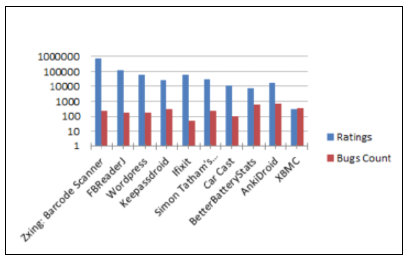
\includegraphics[width=\columnwidth, angle = 0]{images/c1.png}
\caption{XXXX\todo{make into latex}}
\label{fig:userRatings}
\end{figure}


%%% Are these sections even needed?
%\subsection{ZXING Analysis}

%% Talk about how we performed a case study on ZXING

We next decided to perform a case study on a single Android app to better understand how user reviews correlated with reported bugs. Specially, we examined if users are satisfied with application and not asking for many features and also whether the application has many bugs that the user are reporting.


We noticed that the~\emph{ZXING}\footnote{\url{https://play.google.com/store/apps/details?id=com.google.zxing.client.android}} had a high level of user ratings and relatively low bugs count. Therefore, we decided to further analyze this app to understand any possible correlations between these values. We began by extracting user reviews from the ZXING application page in Google Play store and then classify them into feature requests and bug reports. This was accomplished by implementing an algorithm that splits a text into sentences, normalizes them, and compares them with a set of linguistic rules to find if it matches any of them. We used two set of rules for our classification. One is based on the linguistic rules defined by Lacob et al.\cite{Iacob:2013:RAM:2487085.2487094} for feature requests, the other one is based on the linguistic rules they defined for bug reports~\cite{10.1007/978-3-319-05452-0_4}. We adapted the syntax of the rules to work with OpenNLP\footnote{\url{https://opennlp.apache.org/}}, the API we used for part-of-speech tagging. OpenNLP is a machine learning based toolkit for the processing of natural language text.

For issue classification, we created some rules due to assist with classifying the text.Table~\ref{Table:Rule1} shows some examples of linguistic rules for identifying feature requests and an example text that would be a match for each. Table~\ref{Table:Rule2} shows some examples of linguistic rules for identifying bug reports and an example text that would be a match for each. \todo{reword this section}

\begin{table}[h]
\begin{center}
\caption{Examples of rules to identify feature requests}
\label{Table:Rule1}
  \begin{tabular}{ | l | c | c |  } \hline

     \bfseries Rule  & \bfseries Text Match \\ \hline
 
  
	Would be <adjective> if & It would be great if \\ \hline
	Would <adverb> like to <verb> & Would really like to see \\ \hline
	Needs option to & Needs options to share posts \\ \hline
	
  \end{tabular}
  \end{center}
\end{table}



\begin{table}[h]
\begin{center}
\caption{Examples of rules to identify bug reports}
\label{Table:Rule2}
  \begin{tabular}{ | l | c | c |  } \hline

     \bfseries Rule  & \bfseries Text Match \\ \hline
 	
	<adverb> annoying & Incredibly annoying \\ \hline
	Won't <verb> & Files won?t open \\ \hline
	Keeps on crashing & Reader keeps on crashing \\ \hline

  \end{tabular}
  \end{center}
\end{table}


We used Lingpipe\footnote{\url{http://alias-i.com/lingpipe/}} and OpenNLP to create an algorithm that classified the reviews based on those rules. Lingpipe is a toolkit for processing text using computational linguistics. We began by using Lingpipe to split the reviews into sentences. After the review was split into sentences, we normalized each sentence, replacing common misspelled words and abbreviations. When then used OpenNLP to tag the sentence where each word in the review sentence was tagged as a part of speech, e.g. for the text ``it would be great'' the tagger would generate ``<personal\_pronoun> <modal> <verb> <adjective>''.

We ran our algorithm twice for each review we extracted. The first time it compared the review sentence with the linguistic rules defined for feature requests, and if it matched one of the rules, it classified the sentence as a feature request. If a sentence of a review is considered a feature request, then the whole review is marked as such. If any of the sentences is not a feature request, then the review is marked as not a feature request. The second time it did the same, but instead of comparing the sentences with the rules for feature requests, it compared them to the rules for bug reports. After the reviews in the database were classified, we counted the bug reports and feature requests for the application.




\subsection{Discussion}


\todo{add to this}

\section{Public Dataset}
\label{sec:dataset}
%% Is there one we can provide?






\section{Limitations \& Future Work}
\label{sec:threats}


While we feel that our research was profound, there are several possible areas of improvement. In this study, we only analyzed 10 apps which represents only a very tiny portion of all Android apps. Future research may be done to broaden this study to more apps and more genres of apps.




% Compare app genres against one another
% 

% Analyze more apps from more genres

Detecting and defining defects in software is a difficult task. While static analysis tools have demonstrated their benefits in numerous previous works~\cite{7006337, johnson2013don}, they are far from perfect and often produce a large number of false positives or miss actual defects~\cite{chess2004static, Thung:2012:EWD:2351676.2351685}. Another way to determine the amount of bugs in software is through the examination of the application's bug reports. Unfortunately, the absence or presence of errors in bug reports is not always complete. Bugs may not exist in these reports merely because they have yet to be discovered by the users. Less users could mean that less bugs would be reported merely due to the fact that less people were using the app to report the issues. Additionally, duplicate bug entries are often made in bug reporting systems along with entries which are not actually bugs. To combat this, we only considered bug report items which had been considered to be legitimate, and `resolved' in our analysis and ignored defects which had been marked as duplicate, or not actually a bug. Since we only analyzed apps with at least 100,000 downloads, we feel that this offers a reasonable enough sized user based to have found the majority of bugs.





%%% Word matching algorithmbmmmmm                                                                                                                                                                                                                                                                                                                                                                                                                                                                                                                                                                                                                                                                                                                                                                                                                                                                                                                                                                                                                                                                                                                                                                                                                                                                                                                                                                                                                                                                                                                                                                                                                                                                                                                                                                                                                                                                                                                                                                                                                                                                                                                                                                                                                                                                                                                                                                                                                                                                                                                                                                                                                                                                                                                                                                                                                                                                                                                                                                                                                                                                                                                                                                                                                                                                                                                                                                                                                                                                                                                                                                                                                                                                                                                                                                                                                                                                                                                                                                                                                                                                                                                                                                                                                                                                                                                                                                                                                                                                                                                                                                                                                                                                                                                                                                                                                                                                                                                                                                                                                                                                                                                                                                                                                                                                                                                                                                                                                                                                                                                                                                                                                                                                                                                                                                                                                                                                                                                                                                                                                                                                                                                                                                                                                                                                                                                                                                                                                                                                                                                                                                                                                                                                                                                                                                                                                                                                                                                                                                                                                                                                                                                                                                                                                                                                                                                                                                                                                                                                                                                                                                                                                                                                                                                                                                                                                                                                                                                                                                                                                                                                                                                                                                                                                                                                                                                                                                                                                                                                                                                                                                                                                                                                                                                                                                                                                                                                                                                                                                                                                                                                                                                                                                                                                                                                                                                                                                                                                                                                                                                                                                                                                                                                                                                                                                                                                                                                                                                                                                                                                                                                                                                                                                                                                                                                                                                                                                                                                                                                                                                                                                                                                                                                                                                                                                                                                                                                                                                                                                                                                                                                                                                                                                                                                                                                                                                                                                                                                                                                                                                                                                                                                                                                                                                                                                                                                                                                                                                                                                                                                                                                                                                                                                                                                                                                                                                                                                                                                                                                                                                                                                                                                                                                                                                                                                                                                                                                                                                                                                                                                                                                                                                                                                                                                                


%The research would have been given better results if more number of applications were taken into consideration. For this study we have considered only 10 applications which is a very limited number. Also for our research question 2, we considered only 4 applications for each genre. If more number of applications were considered we could have got different results. In Addition, all the applications are written in the same language (Java). We did not explores the code of these apps such as the number of classes, the number of developers, and the experience of developers of these application, to get better results we supposed to select apps the are close in the number of line of codes or the number of developers so that the genre will not be affected by the code.

%When testing our review classification algorithm for Zxing analysis, we used our personal judgment to decide if the algorithm was right or not for identifying a feature request or a bug report. Therefore, the accuracy measures of the algorithm are biased. 








\section{Conclusion}
\label{sec:conclusion}

In this paper, we analyzed the bug history of ten Android apps to better understand how the quality of bug reports can help developers fix bugs sooner, and the relationship between app ratings and bugs. We found a positive correlation between the quality of bug reports and a shorter time to repair the bugs. We also discovered that apps with more bugs typically had a lower user rating.


%that longer, and better bug descriptions 


%In this paper, we analyzed some open source mobile applications, and get the relations between genre, rating, and the quality of bug report. Through analyzing the life cycle of bug, we realize that the users? behavior also affect the quality of mobile application. In this case, it proved that the importance of bug report. We also realize that the difference of user?s patience for different genres. This also decides that there are different decisions of testing and fixing bug in the different genres. For the future work, we can increase the number of mobile applications which are analyzed to get more rich data set. In the same time, we want to make clear for the correlation between length of bug report and the time of fixing. Is there a crest in their correlation? In other words, does the too much information in  bug report effect the developers? understanding for the bug? We hope our research can provide some enlighten for who also analyze this area. 


% ? Add back in for IEE
%%\IEEEpeerreviewmaketitle
\balance
\bibliographystyle{abbrv}
\bibliography{AndroidBugs}

% That's all folks!
\end{document}


%%% 
% Thoughts/Todo
%	Check to see about making this a poster and removing the domain information\
%	Proofread all to make sure it is focused
%	Organize the tables in a proper format







% Project data
%	https://drive.google.com/drive/folders/0B7sYTXKXM0g1fjd1ZWlwQ2hIdzZzbGl6cUU2MWZkRWRYT3doc01FaDdFZmVWaVFHelAyUm8


% http://selab.uos.ac.kr/sacse16/
